\documentclass[11pt]{article}
\usepackage[margin=1in]{geometry}
\usepackage{amsmath,amssymb,amsthm}
\usepackage{graphicx,booktabs,xcolor}
\usepackage[authoryear,round]{natbib}

\usepackage{placeins}
\usepackage{fontspec}
\setmainfont{Times New Roman}
\setsansfont{Arial}
% Use locally cached scalable math fonts at all sizes; no TeX download.
\DeclareFontShape{OML}{cmm}{m}{it}{<->cmmi10}{}
\DeclareFontShape{OMS}{cmsy}{m}{n}{<->cmsy10}{}
\DeclareFontShape{OT1}{cmr}{m}{n}{<->cmr10}{}
\DeclareFontFamily{U}{msb}{}
\DeclareFontShape{U}{msb}{m}{n}{<->msbm10}{}
\DeclareFontFamily{U}{msa}{}
\DeclareFontShape{U}{msa}{m}{n}{<->cmsy10}{}
\renewcommand{\checkmark}{\textnormal{Y}}
\usepackage{hyperref}
\hypersetup{colorlinks=true,linkcolor=blue!50!black,citecolor=blue!50!black,urlcolor=blue!50!black}
\newcommand{\builtdate}{9 October 2026}
\newcommand{\totalruns}{115{,}696}
\newcommand{\ncampaigns}{16}
\newcommand{\CfourHardenLowest}{142}
\newcommand{\CfourHardenSole}{16}
\newcommand{\CfourHardenSolved}{121}
\newcommand{\CfourGrowLowest}{139}
\newcommand{\CfourGrowSole}{11}
\newcommand{\CfourGrowSolved}{119}
\newcommand{\CfourRigidLowest}{155}
\newcommand{\CfourRigidSole}{23}
\newcommand{\CfourRigidSolved}{132}
\newcommand{\CfourSaLowest}{72}
\newcommand{\CfourSaSole}{2}
\newcommand{\CfourSaSolved}{69}
\newcommand{\CfourPcLowest}{64}
\newcommand{\CfourPcSole}{0}
\newcommand{\CfourPcSolved}{63}
\newcommand{\CfourSignGrow}{11 vs 9}
\newcommand{\CfourSignPGrow}{0.82}
\newcommand{\CfourSignRigid}{7 vs 18}
\newcommand{\CfourSignPRigid}{0.043}
\newcommand{\CfourSignSa}{57 vs 5}
\newcommand{\CfourSignPSa}{3.1e-12}
\newcommand{\CfourSignPc}{59 vs 1}
\newcommand{\CfourSignPPc}{1.1e-16}
\newcommand{\CfourInstances}{188}
\newcommand{\CfourUnsolved}{46}
\newcommand{\CfourSquInSquHardenLowest}{28}
\newcommand{\CfourSquInSquHardenSole}{7}
\newcommand{\CfourSquInSquRigidLowest}{20}
\newcommand{\CfourSquInSquRigidSole}{0}
\newcommand{\CfourSquInSquGrowLowest}{21}
\newcommand{\CfourSquInSquGrowSole}{0}
\newcommand{\CfourSquInSquN}{28}
\newcommand{\CfourSquInCirHardenLowest}{16}
\newcommand{\CfourSquInCirHardenSole}{7}
\newcommand{\CfourSquInCirRigidLowest}{19}
\newcommand{\CfourSquInCirRigidSole}{9}
\newcommand{\CfourSquInCirGrowLowest}{11}
\newcommand{\CfourSquInCirGrowSole}{2}
\newcommand{\CfourSquInCirN}{28}
\newcommand{\CfourSquInTriHardenLowest}{27}
\newcommand{\CfourSquInTriHardenSole}{0}
\newcommand{\CfourSquInTriRigidLowest}{29}
\newcommand{\CfourSquInTriRigidSole}{1}
\newcommand{\CfourSquInTriGrowLowest}{24}
\newcommand{\CfourSquInTriGrowSole}{0}
\newcommand{\CfourSquInTriN}{29}
\newcommand{\CfourTriInTriHardenLowest}{19}
\newcommand{\CfourTriInTriHardenSole}{1}
\newcommand{\CfourTriInTriRigidLowest}{24}
\newcommand{\CfourTriInTriRigidSole}{4}
\newcommand{\CfourTriInTriGrowLowest}{22}
\newcommand{\CfourTriInTriGrowSole}{3}
\newcommand{\CfourTriInTriN}{28}
\newcommand{\CfourTriInSquHardenLowest}{10}
\newcommand{\CfourTriInSquHardenSole}{1}
\newcommand{\CfourTriInSquRigidLowest}{18}
\newcommand{\CfourTriInSquRigidSole}{7}
\newcommand{\CfourTriInSquGrowLowest}{19}
\newcommand{\CfourTriInSquGrowSole}{5}
\newcommand{\CfourTriInSquN}{28}
\newcommand{\CfourHexInSquHardenLowest}{15}
\newcommand{\CfourHexInSquHardenSole}{0}
\newcommand{\CfourHexInSquRigidLowest}{17}
\newcommand{\CfourHexInSquRigidSole}{2}
\newcommand{\CfourHexInSquGrowLowest}{15}
\newcommand{\CfourHexInSquGrowSole}{1}
\newcommand{\CfourHexInSquN}{18}
\newcommand{\CfourCirInSquHardenLowest}{27}
\newcommand{\CfourCirInSquHardenSole}{0}
\newcommand{\CfourCirInSquRigidLowest}{28}
\newcommand{\CfourCirInSquRigidSole}{0}
\newcommand{\CfourCirInSquGrowLowest}{27}
\newcommand{\CfourCirInSquGrowSole}{0}
\newcommand{\CfourCirInSquN}{29}
\newcommand{\CsevenHardenLowest}{142}
\newcommand{\CsevenHardenSole}{13}
\newcommand{\CsevenHardenSolved}{125}
\newcommand{\CsevenGrowLowest}{144}
\newcommand{\CsevenGrowSole}{9}
\newcommand{\CsevenGrowSolved}{129}
\newcommand{\CsevenRigidLowest}{155}
\newcommand{\CsevenRigidSole}{16}
\newcommand{\CsevenRigidSolved}{133}
\newcommand{\CsevenSaLowest}{125}
\newcommand{\CsevenSaSole}{6}
\newcommand{\CsevenSaSolved}{115}
\newcommand{\CsevenPcLowest}{72}
\newcommand{\CsevenPcSole}{1}
\newcommand{\CsevenPcSolved}{71}
\newcommand{\CsevenSignGrow}{9 vs 13}
\newcommand{\CsevenSignPGrow}{0.52}
\newcommand{\CsevenSignRigid}{6 vs 14}
\newcommand{\CsevenSignPRigid}{0.12}
\newcommand{\CsevenSignSa}{21 vs 11}
\newcommand{\CsevenSignPSa}{0.11}
\newcommand{\CsevenSignPc}{59 vs 5}
\newcommand{\CsevenSignPPc}{9e-13}
\newcommand{\CsevenInstances}{188}
\newcommand{\CsevenUnsolved}{43}
\newcommand{\CsevenSquInSquHardenLowest}{27}
\newcommand{\CsevenSquInSquHardenSole}{5}
\newcommand{\CsevenSquInSquRigidLowest}{23}
\newcommand{\CsevenSquInSquRigidSole}{1}
\newcommand{\CsevenSquInSquGrowLowest}{21}
\newcommand{\CsevenSquInSquGrowSole}{0}
\newcommand{\CsevenSquInSquN}{28}
\newcommand{\CsevenSquInCirHardenLowest}{16}
\newcommand{\CsevenSquInCirHardenSole}{6}
\newcommand{\CsevenSquInCirRigidLowest}{15}
\newcommand{\CsevenSquInCirRigidSole}{3}
\newcommand{\CsevenSquInCirGrowLowest}{17}
\newcommand{\CsevenSquInCirGrowSole}{4}
\newcommand{\CsevenSquInCirN}{28}
\newcommand{\CsevenSquInTriHardenLowest}{28}
\newcommand{\CsevenSquInTriHardenSole}{0}
\newcommand{\CsevenSquInTriRigidLowest}{29}
\newcommand{\CsevenSquInTriRigidSole}{0}
\newcommand{\CsevenSquInTriGrowLowest}{27}
\newcommand{\CsevenSquInTriGrowSole}{0}
\newcommand{\CsevenSquInTriN}{29}
\newcommand{\CsevenTriInTriHardenLowest}{18}
\newcommand{\CsevenTriInTriHardenSole}{0}
\newcommand{\CsevenTriInTriRigidLowest}{26}
\newcommand{\CsevenTriInTriRigidSole}{4}
\newcommand{\CsevenTriInTriGrowLowest}{24}
\newcommand{\CsevenTriInTriGrowSole}{2}
\newcommand{\CsevenTriInTriN}{28}
\newcommand{\CsevenTriInSquHardenLowest}{14}
\newcommand{\CsevenTriInSquHardenSole}{2}
\newcommand{\CsevenTriInSquRigidLowest}{22}
\newcommand{\CsevenTriInSquRigidSole}{7}
\newcommand{\CsevenTriInSquGrowLowest}{17}
\newcommand{\CsevenTriInSquGrowSole}{3}
\newcommand{\CsevenTriInSquN}{28}
\newcommand{\CsevenHexInSquHardenLowest}{15}
\newcommand{\CsevenHexInSquHardenSole}{0}
\newcommand{\CsevenHexInSquRigidLowest}{16}
\newcommand{\CsevenHexInSquRigidSole}{1}
\newcommand{\CsevenHexInSquGrowLowest}{14}
\newcommand{\CsevenHexInSquGrowSole}{0}
\newcommand{\CsevenHexInSquN}{18}
\newcommand{\CsevenCirInSquHardenLowest}{24}
\newcommand{\CsevenCirInSquHardenSole}{0}
\newcommand{\CsevenCirInSquRigidLowest}{24}
\newcommand{\CsevenCirInSquRigidSole}{0}
\newcommand{\CsevenCirInSquGrowLowest}{24}
\newcommand{\CsevenCirInSquGrowSole}{0}
\newcommand{\CsevenCirInSquN}{29}
\newcommand{\CubesHardenTwelve}{2.942809}
\newcommand{\CubesRigidTwelve}{3.000000}
\newcommand{\CubesGrowTwelve}{2.947506}
\newcommand{\CubesBelow}{none}
\newcommand{\CtauOne}{7}
\newcommand{\CtauHalf}{15}
\newcommand{\CtauQuarter}{18}
\newcommand{\CtauZero}{17}
\newcommand{\CtauN}{40}
\newcommand{\CtauSquares}{3, 4, 2, 0}
\newcommand{\CtauTriangles}{2, 7, 8, 10}
\newcommand{\CbudgetOneHarden}{3}\newcommand{\CbudgetOneRigid}{17}
\newcommand{\CbudgetThreeHarden}{5}\newcommand{\CbudgetThreeRigid}{16}
\newcommand{\CbudgetTenHarden}{9}\newcommand{\CbudgetTenRigid}{16}
\newcommand{\CbudgetN}{20}
\newcommand{\PortRigidSixtyFour}{138}
\newcommand{\PortRigidHarden}{139}
\newcommand{\PortRigidGrow}{137}
\newcommand{\PortSign}{4 vs 3}
\newcommand{\PortP}{1}

\newcommand{\BootHarden}{126--140}
\newcommand{\BootGrow}{123--138}
\newcommand{\BootRigid}{139--153}
\newcommand{\BootSa}{89--107}
\newcommand{\BootPc}{40--56}
\newcommand{\BootDRH}{3 to 24}
\newcommand{\BootDRHMed}{14}
\newcommand{\BootDRHPos}{99\%}
\newcommand{\BootDRG}{5 to 27}
\newcommand{\BootDRGMed}{16}
\newcommand{\BootDRGPos}{99\%}
\newcommand{\BootDGH}{-13 to 9}
\newcommand{\BootDGHMed}{-2}
\newcommand{\BootDGHPos}{30\%}
\newcommand{\EligHarden}{97\%}
\newcommand{\EligGrow}{98\%}
\newcommand{\EligRigid}{100\%}
\newcommand{\EligSa}{94\%}
\newcommand{\EligPc}{56\%}
\newcommand{\RangeSmallHarden}{54}
\newcommand{\RangeSmallGrow}{54}
\newcommand{\RangeSmallRigid}{56}
\newcommand{\RangeSmallSa}{56}
\newcommand{\RangeSmallPc}{47}
\newcommand{\RangeSmallN}{58}
\newcommand{\RangeMidHarden}{50}
\newcommand{\RangeMidGrow}{57}
\newcommand{\RangeMidRigid}{52}
\newcommand{\RangeMidSa}{43}
\newcommand{\RangeMidPc}{20}
\newcommand{\RangeMidN}{70}
\newcommand{\RangeLargeHarden}{38}
\newcommand{\RangeLargeGrow}{33}
\newcommand{\RangeLargeRigid}{47}
\newcommand{\RangeLargeSa}{26}
\newcommand{\RangeLargePc}{5}
\newcommand{\RangeLargeN}{60}
\newcommand{\StepsGrowTwenty}{11{,}500}
\newcommand{\StepsGrowThirty}{11{,}500}
\newcommand{\StepsHardenTwenty}{11{,}500}
\newcommand{\StepsHardenThirty}{11{,}500}
\newcommand{\StepsPcTwenty}{19{,}148}
\newcommand{\StepsPcThirty}{20{,}530}
\newcommand{\StepsRigidTwenty}{11{,}500}
\newcommand{\StepsRigidThirty}{11{,}500}
\newcommand{\StepsSaTwenty}{66{,}854}
\newcommand{\StepsSaThirty}{104{,}043}
\newcommand{\RefEvalsTwenty}{438{,}032}
\newcommand{\RefRatioTwenty}{1.05}
\newcommand{\RefEvalsThirty}{696{,}566}
\newcommand{\RefRatioThirty}{1.07}

\newcommand{\SnapHLower}{17}
\newcommand{\SnapXLower}{36}
\newcommand{\SnapTies}{135}
\newcommand{\SnapP}{0.013}
\newcommand{\SnapHOnly}{6}
\newcommand{\SnapXOnly}{16}
\newcommand{\SnapPReached}{0.052}
\newcommand{\SnapRXLower}{20}
\newcommand{\SnapRRLower}{20}
\newcommand{\SnapRP}{1}
\newcommand{\SnapSquSqu}{6--0}
\newcommand{\SnapRSquSqu}{1--2}
\newcommand{\SnapSquCir}{5--11}
\newcommand{\SnapRSquCir}{10--6}
\newcommand{\SnapSquTri}{0--1}
\newcommand{\SnapRSquTri}{0--0}
\newcommand{\SnapTriTri}{0--8}
\newcommand{\SnapRTriTri}{0--2}
\newcommand{\SnapTriSqu}{6--14}
\newcommand{\SnapRTriSqu}{8--9}
\newcommand{\SnapHexSqu}{0--2}
\newcommand{\SnapRHexSqu}{1--1}
\newcommand{\SnapCirSqu}{0--0}
\newcommand{\SnapRCirSqu}{0--0}
\newcommand{\AreaHLower}{20}
\newcommand{\AreaXLower}{31}
\newcommand{\AreaTies}{137}
\newcommand{\AreaP}{0.16}
\newcommand{\AreaHOnly}{6}
\newcommand{\AreaXOnly}{15}
\newcommand{\AreaPReached}{0.078}
\newcommand{\AreaRXLower}{15}
\newcommand{\AreaRRLower}{14}
\newcommand{\AreaRP}{1}
\newcommand{\AreaSquSqu}{5--1}
\newcommand{\AreaRSquSqu}{2--1}
\newcommand{\AreaSquCir}{9--8}
\newcommand{\AreaRSquCir}{8--4}
\newcommand{\AreaSquTri}{0--1}
\newcommand{\AreaRSquTri}{0--0}
\newcommand{\AreaTriTri}{1--8}
\newcommand{\AreaRTriTri}{0--3}
\newcommand{\AreaTriSqu}{5--11}
\newcommand{\AreaRTriSqu}{5--6}
\newcommand{\AreaHexSqu}{0--2}
\newcommand{\AreaRHexSqu}{0--0}
\newcommand{\AreaCirSqu}{0--0}
\newcommand{\AreaRCirSqu}{0--0}
\newcommand{\BatN}{28}
\newcommand{\BatHReached}{49}
\newcommand{\BatHAll}{14}
\newcommand{\BatHSome}{4}
\newcommand{\BatRReached}{46}
\newcommand{\BatRAll}{14}
\newcommand{\BatRSome}{2}
\newcommand{\BatSqElevenH}{2}
\newcommand{\BatSqElevenR}{0}
\newcommand{\BatSqTwentyNineH}{2}
\newcommand{\BatSqTwentyNineR}{0}
\newcommand{\BatTriTwentyNineH}{1}
\newcommand{\BatTriTwentyNineR}{3}
\newcommand{\LongN}{14}
\newcommand{\LongHardenLowest}{13}
\newcommand{\LongHardenSole}{5}
\newcommand{\LongHardenReached}{12}
\newcommand{\LongGrowLowest}{7}
\newcommand{\LongGrowSole}{0}
\newcommand{\LongGrowReached}{7}
\newcommand{\LongRigidLowest}{8}
\newcommand{\LongRigidSole}{0}
\newcommand{\LongRigidReached}{8}
\newcommand{\LongSaLowest}{9}
\newcommand{\LongSaSole}{1}
\newcommand{\LongSaReached}{9}
\newcommand{\LongPcLowest}{6}
\newcommand{\LongPcSole}{0}
\newcommand{\LongPcReached}{6}
\newcommand{\LongHardenOnlyReachedNewNs}{$n=17$ and $n=26$}
\newcommand{\LongNewHLower}{3}
\newcommand{\LongNewRLower}{0}
\newcommand{\LongNewP}{0.25}
\newcommand{\LongNewN}{11}
\newcommand{\LongHLower}{6}
\newcommand{\LongRLower}{0}
\newcommand{\LongP}{0.031}
\newcommand{\LongHardenSoleNs}{17, 19, 26, 28, 29}
\newcommand{\LongHardenOnlyReachedNs}{17, 19, 26, 29}
\newcommand{\LongSaOnlyReachedNs}{27}
\newcommand{\LongBelow}{0}
\newcommand{\BudOneH}{7}
\newcommand{\BudOneR}{2}
\newcommand{\BudOneP}{0.18}
\newcommand{\BudOneHReached}{17}
\newcommand{\BudOneRReached}{15}
\newcommand{\BudThreeH}{4}
\newcommand{\BudThreeR}{3}
\newcommand{\BudThreeP}{1}
\newcommand{\BudThreeHReached}{18}
\newcommand{\BudThreeRReached}{16}
\newcommand{\BudMoreH}{6}
\newcommand{\BudMoreR}{2}
\newcommand{\BudMoreP}{0.29}
\newcommand{\BudMoreHReached}{18}
\newcommand{\BudMoreRReached}{16}
\newcommand{\BudLvMLH}{3}
\newcommand{\BudLvMMH}{3}
\newcommand{\BudLMPH}{1}
\newcommand{\BudGainH}{4}
\newcommand{\BudLossH}{3}
\newcommand{\BudLvMLR}{3}
\newcommand{\BudLvMMR}{2}
\newcommand{\BudLMPR}{1}
\newcommand{\BudGainR}{5}
\newcommand{\BudLossR}{0}
\newcommand{\BudN}{28}

\IfFileExists{decision.tex}{\newcommand{\DecN}{60}
\newcommand{\DecPilotLower}{2}
\newcommand{\DecRigidLower}{3}
\newcommand{\DecTies}{55}
\newcommand{\DecP}{1}
\newcommand{\DecHLower}{3}
\newcommand{\DecHRLower}{17}
\newcommand{\DecHP}{0.0026}
\newcommand{\DecPicked}{20}
\newcommand{\DecReachedRigid}{40}
\newcommand{\DecReachedHarden}{32}
\newcommand{\DecReachedPilot}{41}
\newcommand{\DecTPicked}{3}
\newcommand{\DecTChanged}{17}
\newcommand{\DecTLower}{2}
\newcommand{\DecTRLower}{3}
}{}
\IfFileExists{refine.tex}{\newcommand{\RefN}{28}
\newcommand{\RefRawHarden}{6}
\newcommand{\RefRawGrow}{19}
\newcommand{\RefRawRigid}{3}
\newcommand{\RefRawSa}{1}
\newcommand{\RefRawPc}{0}
\newcommand{\RefEqHarden}{23}
\newcommand{\RefEqGrow}{20}
\newcommand{\RefEqRigid}{19}
\newcommand{\RefEqSa}{17}
\newcommand{\RefEqPc}{4}
\newcommand{\RefPolHarden}{24}
\newcommand{\RefPolGrow}{20}
\newcommand{\RefPolRigid}{18}
\newcommand{\RefPolSa}{14}
\newcommand{\RefPolPc}{2}
}{}
\newcommand{\MechSquSquHardenMove}{0.45}
\newcommand{\MechSquSquHardenTurn}{23}
\newcommand{\MechSquSquHardenTilt}{0.13}
\newcommand{\MechSquSquHardenOrder}{0.53}
\newcommand{\MechSquSquRigidMove}{0.36}
\newcommand{\MechSquSquRigidTurn}{5}
\newcommand{\MechSquSquRigidTilt}{0.11}
\newcommand{\MechSquSquRigidOrder}{0.81}
\newcommand{\MechSquCirHardenMove}{0.52}
\newcommand{\MechSquCirHardenTurn}{21}
\newcommand{\MechSquCirHardenOrder}{0.24}
\newcommand{\MechSquCirRigidMove}{0.43}
\newcommand{\MechSquCirRigidTurn}{22}
\newcommand{\MechSquCirRigidOrder}{0.37}
\newcommand{\MechSquTriHardenMove}{0.35}
\newcommand{\MechSquTriHardenTurn}{23}
\newcommand{\MechSquTriHardenTilt}{0.06}
\newcommand{\MechSquTriHardenOrder}{0.29}
\newcommand{\MechSquTriRigidMove}{0.17}
\newcommand{\MechSquTriRigidTurn}{9}
\newcommand{\MechSquTriRigidTilt}{0.03}
\newcommand{\MechSquTriRigidOrder}{0.20}
\newcommand{\MechTriTriHardenMove}{0.53}
\newcommand{\MechTriTriHardenTurn}{30}
\newcommand{\MechTriTriHardenTilt}{0.00}
\newcommand{\MechTriTriHardenOrder}{0.28}
\newcommand{\MechTriTriRigidMove}{0.28}
\newcommand{\MechTriTriRigidTurn}{18}
\newcommand{\MechTriTriRigidTilt}{0.00}
\newcommand{\MechTriTriRigidOrder}{0.23}
\newcommand{\MechTriSquHardenMove}{0.62}
\newcommand{\MechTriSquHardenTurn}{28}
\newcommand{\MechTriSquHardenTilt}{0.29}
\newcommand{\MechTriSquHardenOrder}{0.10}
\newcommand{\MechTriSquRigidMove}{0.45}
\newcommand{\MechTriSquRigidTurn}{26}
\newcommand{\MechTriSquRigidTilt}{0.21}
\newcommand{\MechTriSquRigidOrder}{0.06}
\newcommand{\MechHexSquHardenMove}{0.13}
\newcommand{\MechHexSquHardenTurn}{15}
\newcommand{\MechHexSquHardenTilt}{0.07}
\newcommand{\MechHexSquHardenOrder}{0.44}
\newcommand{\MechHexSquRigidMove}{0.11}
\newcommand{\MechHexSquRigidTurn}{7}
\newcommand{\MechHexSquRigidTilt}{0.00}
\newcommand{\MechHexSquRigidOrder}{0.71}
\newcommand{\MechSoleN}{5}
\newcommand{\MechSoleTiltH}{0.45}
\newcommand{\MechSoleTiltR}{0.28}
\newcommand{\MechSoleMore}{5}
\newcommand{\MechTriFailN}{4}
\newcommand{\MechTriFailMoveH}{0.54}
\newcommand{\MechTriFailMoveR}{0.30}

\newcommand{\CtenRegisteredP}{0.5}


\title{Soft-to-Rigid: Shape Continuation as an Alternative Search\\ for Packing Congruent Shapes}
\author{Yohei Nakajima\\\small Affiliation, corresponding contact and ORCID: author confirmation pending}
\date{Journal preparation draft, 2 November 2026}

\setlength{\emergencystretch}{1em}
\begin{document}
\maketitle
\begin{center}\fbox{\parbox{0.92\linewidth}{\small\textbf{Author-review draft; not submitted.} Submission identity, funding/conflicts, rights, AI-use details and companion-note status require author confirmation. The public arXiv v1 and historical study artifacts are preserved.}}\end{center}

\begin{abstract}
Hardening searches for dense packings by starting congruent pieces as their inscribed disks and continuously deforming them into prescribed polygons while compressing the container. Shape evolution is established in packing physics; our contribution is a controlled study of this finite-container optimization path and its failure boundaries. We compare hardening, rigid starts, growth, simulated annealing and perturbation--compression across seven families and \CsevenInstances{} instances. Gradient paths have equal step budgets; the two in-house baselines use reference-hardening pair-evaluation budgets, with measured overshoot and separate postprocessing costs. Tuned rigid starts attain the lowest container size most often overall. Hardening reaches particular square packings missed by the other tested searches within the stated run counts. A targeted higher-budget follow-up adds two such best-known successes, while identifying reused runs explicitly. At equal nominal total run budget, a mixed hardening--rigid allocation solves \PortRigidHarden{} instances versus \PortRigidSixtyFour{} for doubled rigid search; this does not demonstrate an advantage or equivalence. A preregistered pilot policy on four additional families likewise shows no detected gain. Exploratory ablations and selected replay measurements describe different search behavior without identifying a causal mechanism. Versioned plans, run outputs, saved analyses and selected replays support inspection. These results characterize an alternative search path under the tested tuning and budget design; they establish neither general competitiveness nor a validated rule for allocating a fixed compute budget.

\end{abstract}
\noindent\textbf{Keywords:} geometric packing; shape continuation; stochastic search; computational experiments; reproducibility

\section{Introduction}
How small a container holds $n$ copies of a given shape? For unit squares in a square the question goes back to \citet{erdosgraham}; catalogues now cover squares, triangles, hexagons and cubes in squares, triangles, circles and cubes \citep{friedmancenter,squaresproject}, and most entries are best known packings found by search rather than proved optimal. Most searches move rigid pieces: simulated annealing \citep{kirkpatrick}, perturbation and compression \citep{Gensane2004,gensane}, growing the pieces in size \citep{lubachevsky}, overlap minimisation in a shrinking container \citep{Umetani2009,Gardeyn2025}, or global solvers on exact non-overlap models \citep{Berthold2026}.

This paper changes the pieces instead. \emph{Hardening} starts every piece as the disk inscribed in it, compresses the disks under inward pressure on the container, and deforms them into the target shape while the pressure continues. It is graduated non-convexity \citep{blake} applied to geometry: a disk has no orientation, so the pieces are already densely packed when their corners appear and rotation becomes a choice. The shape family it moves along, a polygon dilated by a disk at fixed inradius, is not new: it is the spheropolygon of discrete-element modelling \citep{AlonsoMarroquin2008}, and \citet{Jin2015} moved dense periodic packings along its 3D analogue in both directions between tetrahedra and spheres. Our contribution is a controlled finite-container comparison of this optimisation path toward a prescribed polygon, with explicit tuning, budget and postprocessing limits (Section~\ref{sec:related}); it is not a claim to have invented shape evolution. On squares it recovers several classical packings from random starts, and the earlier companion project reported a twelve-cube feasible packing \citep{softtorigidpacking}; that prior discovery is not a new record of the controlled study here.

Here we ask whether hardening is a search worth running alongside existing ones. We compare three paths through shape space (hardening, growing, and rigid pieces on the same schedule) and two classical baselines on seven families of shapes and containers (\totalruns{} stored run records in \ncampaigns{} search campaigns, including deterministic C16 reuse rather than that many independent trials, plus one tightening-only campaign), with the explicit step and pair-evaluation budget design of Section~\ref{sec:method} and comparable grid-search effort. Since a packing search is judged by the best packing it finds, the comparison is by the \emph{lowest} container size each method reaches in a fixed number of runs, after constrained numerical tightening; the procedure being compared is the batch of runs, not a single run \citep{Birattari2005}. Our findings:
\begin{itemize}\itemsep1pt
\item Hardening is not a better default. Untuned, it looked better than rigid starts; tuned with comparable effort, rigid starts reach the lowest size most often over the seven families (Table~\ref{tab:main}).
\item It is a different search. On squares in a square it reaches the lowest size on \CsevenSquInSquHardenLowest{} of \CsevenSquInSquN{} instances and is the only method that low on \CsevenSquInSquHardenSole, including Trump's $n=11$ and Wainwright's $n=19$ packings, which rigid starts reach in none of our campaigns. In a targeted follow-up campaign at ten times the budget it is the only one of five methods to reach the best known packings for \LongHardenOnlyReachedNewNs; it also does so at $n=19$ and 29, but those hardening and rigid runs repeat an earlier campaign (Section~\ref{sec:learned}).
\item Exploratory ablations show that neither the disk-compressed start nor matched area growth reproduces hardening's pattern (Table~\ref{tab:ablate}), consistent with an effect of the gradual path; the pre-registered tests on squares in a square are inconclusive, and hardening's unique packings end with more tilted pieces (Figure~\ref{fig:mechanism}) without that isolating orientation as the cause.
\item The bias has a cost. Hardening is worse on triangles and on four families withheld from tuning and method analysis, apart from the disclosed preregistration geometry smoke tests, and the pilot policy we tested, which chooses the path per instance from 8 runs of each, showed no detected advantage over always starting rigid (Table~\ref{tab:decision}). An earlier indication that it gains more from longer runs did not replicate.
\end{itemize}
Search campaigns were planned in writing before they ran; amendments, exploratory analyses and post-hoc checks are identified separately. Raw outputs and saved analyses are versioned; selected best/hit trajectories have decimated replays. The original event export covers C00--C10, with later analyses also consuming campaign files directly. Online Resource 1 maps the evidence and distinguishes saved-data inspection from rerunning optimization. Section~\ref{sec:matters} gives the practical rule that follows and describes downstream reuse of the earlier release.

\section{Related work}\label{sec:related}
\paragraph{Changing shape during a packing simulation.} Hard-particle physics has long changed particle shape during a run. The event-driven molecular dynamics of \citet{Donev2005a}, which generalises Lubachevsky--Stillinger growth \citep{lubachevsky}, explicitly allows time-dependent particle shapes. ``Digital alchemy'' \citep{vanAnders2015,Geng2019} treats shape parameters as thermodynamic variables sampled by Monte Carlo shape moves, to design shapes for a target structure. Closest to our parametrisation, \citet{Jin2015} take spherotetrahedra (a tetrahedron dilated by a ball, with a roundness ratio defined relative to a tetrahedron of the same inscribed sphere) and evolve dense periodic packings along that family in both directions: from tetrahedron packings toward spheres, and, in an ``inverse evolution'', from sphere packings toward tetrahedra. Superdisk and superball families \citep{Jiao2008,Jiao2009}, truncation families \citep{Engel2012} and rounded cubes in spherical confinement \citep{Wang2018} interpolate between round and faceted shapes, but packings are computed separately at each shape. Minkowski rounding is standard in discrete-element modelling as spheropolygons \citep{AlonsoMarroquin2008,GalindoTorres2010}, where it smooths contact geometry but is held fixed. Starting round and becoming faceted is therefore not new. What hardening adds is the setting: the same inradius-preserving family used as an optimisation homotopy toward a prescribed polygon inside a finite container, scored by the smallest container reached and compared against tuned rigid searches with ablations of the path. It is an instance of graduated non-convexity and continuation \citep{blake,AllgowerGeorg1990}, for which there is theory on when following a path beats a cold start and when it need not \citep{Mobahi2015,Hazan2016}.

\paragraph{Disks as a stand-in for polygons.} In operations research, inscribed circles appear as relaxations or surrogates: QP-Nest \citep{Jones2014} bounds nesting problems by enforcing non-overlap only on inscribed circles, and sparrow \citep{Gardeyn2025} builds its overlap proxy from inscribed ``poles''. In facility layout and floorplanning, modules are first modelled as circles and then converted to exact shapes in a second stage \citep{AnjosVannelli2002,Luo2008}. These use circles as a fixed surrogate or as a one-shot initial solution. We deform each piece continuously from its inscribed disk while the container is compressed, and test separately whether the disk-compressed start or the gradual path is responsible for any effect (campaign C11).

\paragraph{Packing in containers.} Phi-functions \citep{Bennell2010,Romanova2018} and separating-line programs \citep{Peralta2018} give exact non-overlap models; our tightening step is a separating-line program of this kind. Overlap minimisation in a shrinking container dominates irregular strip packing \citep{Umetani2009,Imamichi2009,Egeblad2007,Gardeyn2025}, with jostling as a constructive alternative \citep{Dowsland1998}; analytical placers replace overlap with a smooth density penalty of increasing weight \citep{Lu2015}; and gradient descent on poses with an adaptively shrinking container has recently been applied to irregular 3D objects \citep{Gupta2026}. Our energy is of this family; what differs is that the pieces' shapes change along the way.

\paragraph{Records.} Best known packings of equal pieces come from Friedman's survey and Packing Center \citep{friedmansurvey,friedmancenter}, the Squares Project \citep{squaresproject} and Packomania \citep{packomania}. Record-finding methods include billiards and growth \citep{lubachevsky,LubachevskyGraham1997}, perturbation--compression \citep{Gensane2004,gensane}, perturbation-based thresholding search \citep{Lai2023}, periodic adaptive-shrinking-cell and divide-and-concur optimisation \citep{TorquatoJiao2009,Kallus2010}, global MINLP solvers \citep{Berthold2026}, and LLM-driven program search \citep{Novikov2025,Georgiev2025,hyra}. \citet{Berthold2026} solve regular polygons in regular polygons and Platonic solids in Platonic solids for $n\le30$; their supplement lists 12 cubes at $2.94281$ (Friedman's 1998 value), and Hyra \citep{hyra} later reports $2.93277$. Records for squares in a square at larger $n$ ($n\ge88$) continue to fall to an iterative ``shrink-hopping'' search with exact certificates \citep{squish}.

\paragraph{Evaluating stochastic searches.} A record search is used for the best packing it finds, so we compare the lowest size each method reaches in a fixed number of runs. \citet{Birattari2005} point out that the best of $N$ runs of an algorithm is one sample from a different algorithm, $N$ restarts of the first, and that this algorithm should be judged by its behaviour over repeated batches, not by one batch's best. We therefore treat ``32 runs of a method'' as the procedure under comparison, report repeated independent batches where we have them, and use resampling only as a sensitivity check, in the spirit of performance profiles and time-to-target plots \citep{Dolan2002,Aiex2007,Hansen2021}. \citet{Lai2023} report best, mean and success rate over 20 runs against Packomania; we add matched budgets, matched tuning effort and pre-registered decision rules.

\section{Method}\label{sec:method}
\paragraph{Pieces and paths.} A piece is a regular polygon $P$ with unit side and inradius $\rho$ (a unit square, triangle or hexagon), or a unit-diameter disk. Its \emph{shape state} is
\[
P(\gamma,\tau)=\gamma\big[(1-\tau)\,P\;\oplus\;\tau\rho\,D\big],
\]
the polygon scaled about its incenter, dilated by a disk of radius $\tau\rho$ (a spheropolygon \citep{AlonsoMarroquin2008}), and scaled by $\gamma$. At $\tau=1$ it is the inscribed disk, at $\tau=0$ the polygon, and for $\gamma\le1$ every state lies inside the polygon, so moving toward $(\gamma,\tau)=(1,0)$ only grows the piece. Two facts describe what the family does. Its support function is
\[
h_{P(\gamma,\tau)}(u)=\gamma\big[(1-\tau)\,h_P(u)+\tau\rho\big],
\]
for a unit direction $u$, so the dependence of a piece's extent on its orientation is scaled down by $(1-\tau)$: rotating a nearly round piece barely changes the energy, and orientation becomes a decision only late in the path. And since $A(P)=\tfrac12\,\mathrm{perimeter}\cdot\rho$, its area at $\gamma=1$ is
\[
A(\tau)=A(P)-\big[A(P)-\pi\rho^2\big]\tau^2 ,
\]
so a hardening piece gains the area outside its inscribed disk, $21\%$ of a square, $9\%$ of a hexagon and $40\%$ of a triangle. A \emph{path} is a schedule for $(\gamma,\tau)$ during the middle phase of a run (Figure~\ref{alg:run}). We compare three:
\begin{itemize}\itemsep0pt
\item \textbf{harden}: $\gamma=1$, $\tau:1\to0$ (disks harden into polygons);
\item \textbf{grow}: $\tau=0$, $\gamma:\gamma_0\to1$ (rigid polygons grow, as in Lubachevsky--Stillinger \citep{lubachevsky});
\item \textbf{rigid}: $(\gamma,\tau)=(1,0)$ throughout, on the same schedule;
\end{itemize}
and two classical baselines on rigid pieces: \textbf{sa}, Metropolis simulated annealing over poses and container size \citep{kirkpatrick}, and \textbf{pc}, perturbation--compression \citep{Gensane2004,gensane} (shrink, relax, perturb on failure). Two further paths serve as ablations: \textbf{snap} compresses disks exactly as harden does and then switches to the polygons at once ($\tau:1\to0$ in one step), and \textbf{grow-area} keeps rigid polygons whose area follows hardening's area schedule ($\tau=0$, $\gamma^2=1-(1-\pi\rho^2/A)\,t^2$ with $t:1\to0$).

\paragraph{Energy.} The container (square, equilateral triangle or circle) is centred at the origin with size $L$: side length for a square/equilateral triangle, radius for a circle. For poses $(x_i,y_i,\theta_i)$,
\[
E=\sum_{i<j}\big(2r-\operatorname{sd}_{ij}\big)_+^2+\sum_{i}\sum_{v}\big(\text{wall violation of }v\big)_+^2+\mu L,
\]
where $r=\gamma\tau\rho$, $\operatorname{sd}_{ij}$ is the signed distance between the cores (exact vertex--edge distance when apart, minus the separating-axis penetration depth when overlapping) and $v$ ranges over core vertices. The term $\mu L$ is inward pressure. Positions, angles and $L$ follow momentum gradient descent with analytic gradients and decaying Gaussian noise. In 3D the same holds for cubes with quaternion orientations and the 15-axis separating test \citep{softtorigidpacking}.

\begin{figure}[t]
\centering\fbox{\begin{minipage}{0.92\linewidth}\small
\textbf{One gradient-path run.} Let $B$ denote the budget multiplier; base compression, morph and settling lengths are $n_C,n_M,n_S=2500,7500,1500$ steps.
\begin{enumerate}\itemsep0pt
\item Initialize random poses in a container of area $3.2$ times the pieces' area; set $(\gamma,\tau)$ to the path start.
\item Compress for $Bn_C$ steps with pressure $3\mu$ and decaying noise.
\item Follow the path for $Bn_M$ steps: update $(\gamma,\tau)$ with normalized progress, and take momentum steps at pressure $\mu$ with decaying noise.
\item Settle the final pieces for $Bn_S$ steps with no noise, decaying pressure as $\mu 10^{-4s/(Bn_S)}$.
\item Legalise by scaling centres apart until the pair-overlap tolerance is met, then measure the smallest container.
\end{enumerate}
\end{minipage}}
\caption{One gradient-path run with the step schedule used in the study}\label{alg:run}
\end{figure}

\paragraph{Step details.} Each momentum step updates velocities as $v\leftarrow0.85\,v-0.04\,\nabla E$ (container size: $v_L\leftarrow0.85\,v_L-0.02\,(\mu+\partial E/\partial L)$), caps a piece's translation step at $0.03\sqrt2\,R$ ($R$ the circumradius) and its rotation at $0.03$ rad, then adds Gaussian noise. With noise multiplier $\nu$ (Appendix, frozen settings), the positional noise is $0.015\,\nu\,(1-u)$ during compression and $0.004\,\nu\,(1-u)$ during the path, where $u\in[0,1]$ is progress through the phase, and the angular noise is $1.5$ times the positional noise. The implementation is \texttt{engine/engine2d.js}.

\begin{figure}[t]\centering
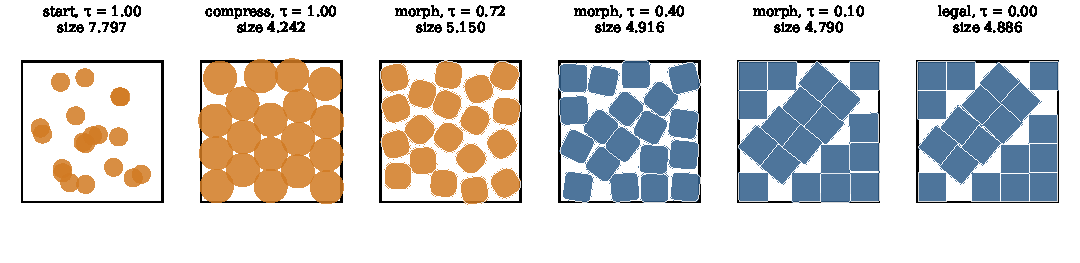
\includegraphics[width=\linewidth]{figures/strip_squ19}\\[2pt]
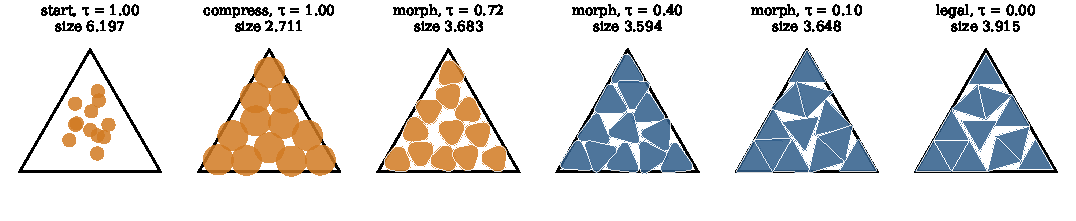
\includegraphics[width=\linewidth]{figures/strip_tri12}
\caption{Two hardening runs (C07). Top: 19 squares; disks are compressed, harden into squares, and settle into Wainwright's packing (side $3+4\sqrt2/3$), which no other method reached in 32 runs. Bottom: the best of 32 hardening runs for 12 triangles in a triangle ends at $3.915$, while rigid and snap starts reach the best known $3.879$; the triangles that emerge from the near-hexagonal disk arrangement keep orientations that do not tile. These are selected decimated replays from versioned campaign files. The triangle size $3.915$ is the legalised simulator endpoint before tightening.}\label{fig:strip}\label{fig:tristrip}
\end{figure}

\paragraph{Legalisation, tightening and certification scope.} Penalties tolerate small overlaps, so every run is \emph{legalised}: centres are scaled apart about their mean until no pair overlaps by more than $10^{-12}$ under the separating-axis test, and the smallest container (translation free) is measured. Near-best runs are then \emph{tightened} by constrained numerical optimisation: minimise $L$ over poses and one separating line (plane) per nearby pair \citep{Peralta2018}, with every vertex inside the container, by SLSQP \citep{kraft} in trust-region outer iterations, keeping a step only if the independently legalised size decreases. Tightening is a local method and gives no optimality guarantee; it only removes the slack a penalty method leaves. The below-catalogue certification route (not applied to every numerically reached catalogue value) spreads a tightened packing below a catalogue value to a clearance of $10^{-6}$ and checks it twice: in floating point, and in exact rational arithmetic. The exact check uses rational rotations from $\tan(\theta/2)$, replaces each piece by a rational polygon scaled by $1+10^{-8}$ and proves, in $\mathbb{Q}(\sqrt3)$, that this polygon contains the true unit polygon with margin $10^{-9}$, and exhibits a rational separating direction for every pair. The current exact 2D checker supports circles, triangles, squares and hexagons; it does not certify the pentagon/octagon families in C15. A numeric reached classification is not an exact certificate or an optimality proof. No below-catalogue claim folder was produced by this controlled study. Online Resource~1 checks four separately enlarged square witnesses; those certificates do not establish feasibility at their original contact objectives.

\paragraph{Budgets.} A run's budget is its number of steps: every gradient path takes $11{,}500\,B$ steps. Pair evaluations then differ by path, since soft pieces have more near neighbours: at $n=20$ squares in a square a hardening run makes about $1.2\times$ the pair evaluations of a rigid run (Table~\ref{tab:diag} in the appendix), which, if anything, favours hardening. The two baselines are stopped once their pair evaluations exceed those of a reference hardening run at the same $n$ (one fixed seed, with the baseline's own pressure and noise settings); for squares in a square this reference is \RefEvalsTwenty{} pair evaluations at $n=20$ and \RefEvalsThirty{} at $n=30$, $\RefRatioTwenty$ and $\RefRatioThirty$ times the mean of the 32 tuned hardening runs. Simulated annealing adds a final short gradient relaxation; perturbation--compression stops at the end of a relaxation. For the square-in-square diagnostics in Table~\ref{tab:diag}, mean pair evaluations divided by the saved reference allowance are $1.02476$ and $1.02520$ for annealing at $n=20,30$, respectively, and $1.57588$ and $1.68891$ for perturbation--compression. These are means for those two cells, not global maxima. In recorded simulator wall-clock time on one core of the study machine (Node.js; tightening excluded), hardening was the fastest of the five methods in the two square-in-square diagnostic cells, $n=20$ and 30 (Table~\ref{tab:diag}). This timing observation is specific to the measured machine and simulator workload. It excludes tuning, repeated reference runs, postprocessing and verification, so it does not establish equal end-to-end cost or general wall-clock superiority.

\paragraph{Endpoint and assistance definitions.} For non-truncated values, a run reaches the catalogue when its selected size is no more than the value plus $10^{-9}$. For truncated values, the ledger verdict uses a gap strictly below the stored printed-precision tolerance (default $10^{-5}$), while the later saved statistical/policy code uses size no greater than value plus tolerance. Lowest-size ties use relative $10^{-9}$, with an additional $10^{-12}$ absolute allowance in the C07 descriptive count code; C15 strict-lower comparisons use $x<y(1-10^{-9})$. These numeric rules do not certify equality or optimality. Substantive AI assistance in implementation, analysis, writing and preparation review is described in Statements and Declarations.

\section{From squares to cubes}\label{sec:story}
The method was developed on unit squares in a square, where records are dense and audited \citep{squaresproject,friedmansurvey}. With the original schedule, hardening reaches Trump's packing for $n=11$ \citep{trump} after tightening (to within $10^{-14}$) in 4 of 80 random starts at three times the base budget and 2 of 80 at the base budget; rigid starts with the same schedule reach it in none of 80 at either budget (campaign C00).

An earlier note by the author, \emph{Twelve unit cubes in a cube of side 2.93152} (submitted to Geombinatorics; current editorial status unconfirmed), reported a feasible packing of 12 unit cubes in a cube of side $2.9315185$. The public code and certificate are separately available \citep{softtorigidpacking}. Its public repository compares this bound with the catalogued Hyra value $2.9327718$ and Friedman's 1998 value $2.94281$ \citep{hyra,friedmancubes}; these are historical comparator snapshots, not a current priority adjudication. The author's public build log flags novelty relative to Haowei Lin's arrangement as disputed \citep{prioritycontext2026}. We therefore use the earlier bound only as context and make no new-record or undisputed-priority claim; its priority is unnecessary to the controlled comparison here. Campaign C05 repeats the cube experiment with three gradient paths and two settings at the earlier bound's search budget (Table~\ref{tab:cubes}). Hardening has the lowest side of the three paths at $n=11$, 12 and 13 under both settings, all paths reach Friedman's $n=9$ packing \citep{friedmancubes}, and with tuned settings hardening and rigid starts also reach his $n=10$ packing $2+1/\sqrt2$, which the original schedule never did. Rigid starts end at the trivial side 3 for $n\ge12$. In these 32 seeds nothing went below a catalogue value: the best side at $n=12$ is \CubesHardenTwelve{} (grow \CubesGrowTwelve, rigid \CubesRigidTwelve), while the earlier feasible bound was reported from one of 192 runs. At $n=13$ hardening reaches $2.956145$, consistent with Friedman's $2.956+$ \citep{friedmancubes} to the precision printed.

\begin{table}[t]\centering\small
\begin{tabular}{rrrrrrrr}
\toprule
 & & \multicolumn{3}{c}{original settings} & \multicolumn{3}{c}{2D-tuned settings}\\
$n$ & reference & harden & grow & rigid & harden & grow & rigid\\
\midrule
9 & 2.70711 & \textbf{2.70711} & \textbf{2.70711} & \textbf{2.70711} & \textbf{2.70711} & \textbf{2.70711} & \textbf{2.70711}\\
10 & 2.70711 & 2.76777 & 2.76777 & 2.89443 & \textbf{2.70711} & 2.76777 & \textbf{2.70711}\\
11 & 2.88295 & \textbf{2.89443} & 2.91739 & 2.91899 & 2.91250 & 2.91328 & 2.94281\\
12 & 2.93277 & 2.94301 & 2.98587 & 3.00000 & \textbf{2.94281} & 2.94751 & 3.00000\\
13 & 2.95600 & 2.99497 & 3.00000 & 3.00000 & \textbf{2.95615} & 3.00000 & 3.00000\\
14 & 2.98995 & \textbf{3.00000} & \textbf{3.00000} & \textbf{3.00000} & \textbf{3.00000} & \textbf{3.00000} & \textbf{3.00000}\\
\bottomrule
\end{tabular}
\caption{Cubes in a cube (C05): lowest side over 32 runs at the prior search budget, after tightening. The reference column excludes the prior reported $n=12$ feasible bound ($2.93152$), from a separate 192-start search; this is not a current-study catalogue target. Bold: lowest in the row.}
\label{tab:cubes}
\end{table}


Two results made the broader question worth asking. Rigid starts in these first experiments used the hardening schedule untouched, so they were never given a fair chance. And squares in a square may be special: many of its best packings tilt a few squares against their neighbours, exactly the configurations a late commitment to orientation should help with.

\section{A wider test}\label{sec:breadth}
\paragraph{Design.} Seven families: unit squares in a square, a circle and a triangle; unit triangles in a triangle and a square; unit hexagons in a square; and, as a control, unit-diameter disks in a square, where hardening changes nothing because a disk is already a disk. Best known values come from the Squares Project \citep{squaresproject}, Friedman's catalogue \citep{friedmancenter} and Packomania \citep{packomania}; truncated catalogue values (``$2.956+$'') count as reached within their printed precision. All $n$ from 2 to 30 (to 20 for hexagons) are used except five reserved for tuning, \CsevenInstances{} instances in all.

Each method was tuned twice, first by median gap on held-out instances (C01--C03; a $3\times3$ grid, extended past its edge by a fixed rule, so harden, sa and pc saw 27 settings and grow and rigid 18), then by the lowest size reached (C06; one $3\times3$ grid per method, 16 runs per setting on each of eight held-out instances of squares in a square and in a circle and triangles in a square and in a triangle, scored by the mean over instances of the lowest of the 16 runs). The second round used larger instances ($n>30$) than the test set, so its settings may be less suited to small $n$; Table~\ref{tab:range} breaks the results down by $n$. Each method then ran 32 times per instance at the nominal allocation described in Section~\ref{sec:method}, and in each instance and method the best run (if within 2\% of the best known value) and any run within $2\cdot10^{-3}$ of it, at most three, were tightened. Plans recorded intended comparisons, with the registration-timing limits and amendments documented in Online Resource~1; the disclosed C15 geometry smoke tests preceded its plan. Changes after a campaign started are recorded as amendments.

\paragraph{Result.} Table~\ref{tab:main} counts, per family, the instances on which each method's lowest size is the lowest of all five. Rigid starts reach the lowest size most often overall (\CsevenRigidLowest{} instances, against \CsevenGrowLowest{} for grow and \CsevenHardenLowest{} for harden) and reach the best known value most often (\CsevenRigidSolved{} against \CsevenGrowSolved{} and \CsevenHardenSolved{}). As a check of sensitivity to the particular seeds, we resampled each instance's 32 runs with replacement (1000 times) and recounted. Within each resample, rigid's count exceeds hardening's in \BootDRHPos{} of resamples (difference \BootDRH, 95\% range) and grow's in \BootDRGPos{}, while grow against harden goes either way (\BootDGH). This measures sensitivity to the seed pool on these instances, not uncertainty about future campaigns: a resample cannot contain a run better than the ones observed, it omits a cell's single best run with probability $(31/32)^{32}\approx0.36$, which is why every method's resampled count is lower than its observed one, and tightened sizes are fixed by the original pool rather than re-selected in each resample. Over instances solved by exactly one of the two, harden against rigid is \CsevenSignRigid{} (exact sign test, $p=\CsevenSignPRigid$). C04 and C07 specified one-sided tests in favor of hardening. For C07 against rigid starts the registered value is $p_1=0.979305$, so that directional hypothesis is not supported; the descriptive two-sided value is $p_2=0.115318$. Later C11--C13, C15 and C16 plans specify two-sided tests. With the doubled-minimum-tail convention, $p_2\le2p_1$ for either one-sided direction; reversing the observed direction makes the registered $p_1$ large, not this inequality false. Online Resource~1 reports the omitted C04/C07 grow, annealing and perturbation--compression comparisons and the remaining plan-specified tests. Simulated annealing improved most from tuning for the lowest point; perturbation--compression stays far behind at this budget, partly because its best run was within reach of tightening on only \EligPc{} of instances (against \EligHarden{} to \EligRigid{} for the gradient paths; Table~\ref{tab:diag}). The similar eligibility fractions for rigid and hardening limit one obvious source of asymmetry, but alone do not establish that tightening cannot affect their relative ordering. To check whether it decides the rest of the comparison, campaign C14 tightened the three best runs of every method on the \RefN{} instances fixed in advance for C13 ($n=11,17,23,29$ per family; hexagons $n=8,12,16,20$), with no eligibility condition. Under equal tightening the baselines gain a few instances and the order on these \RefN{} instances, where hardening happens to lead, is unchanged (Table~\ref{tab:refine}); the subset is too small to rule out larger changes for sa and pc elsewhere. Without any tightening the order is different, so comparisons of penalty methods on legalised sizes alone would mislead.

\begin{table}[t]\centering\small
\begin{tabular}{lccccc}\toprule
treatment & harden & grow & rigid & sa & pc\\\midrule
no tightening & \RefRawHarden & \RefRawGrow & \RefRawRigid & \RefRawSa & \RefRawPc\\
C07 policy (within 2\%, up to 3 runs) & \RefPolHarden & \RefPolGrow & \RefPolRigid & \RefPolSa & \RefPolPc\\
equal (best 3 runs of every method) & \RefEqHarden & \RefEqGrow & \RefEqRigid & \RefEqSa & \RefEqPc\\\bottomrule
\end{tabular}
\caption{Instances on which each method's lowest size is the lowest of all five, on the \RefN{} instances of C14, under three tightening treatments of the same C07 runs.}\label{tab:refine}
\end{table} No run went below a published value, and \CsevenUnsolved{} instances were solved by no method. The median-tuned comparison (C04, Table~\ref{tab:median}) also puts rigid starts first.

\begin{table}[t]\centering\small
\begin{tabular}{lrccccc}
\toprule
family & $N$ & \textbf{harden} & \textbf{grow} & \textbf{rigid} & \textbf{sa} & \textbf{pc} \\
\midrule
squares in square & 28 & \textbf{27 (5)} & 21 & 23 (1) & 21 & 17 \\
squares in circle & 28 & 16 (6) & \textbf{17 (4)} & 15 (3) & 14 (2) & 8 \\
squares in triangle & 29 & 28 & 27 & \textbf{29} & 24 & 8 \\
triangles in triangle & 28 & 18 & 24 (2) & \textbf{26 (4)} & 19 & 10 \\
triangles in square & 28 & 14 (2) & 17 (3) & \textbf{22 (7)} & 9 & 5 \\
hexagons in square & 18 & 15 & 14 & \textbf{16 (1)} & 14 (2) & 9 \\
circles in square (control) & 29 & \textbf{24} & \textbf{24} & \textbf{24} & \textbf{24 (2)} & 15 (1) \\
\midrule
all & 188 & 142 (13) & 144 (9) & \textbf{155 (16)} & 125 (6) & 72 (1) \\
reached best known & & 125 & 129 & 133 & 115 & 71 \\
\bottomrule
\end{tabular}
\caption{Lowest point by family (C07; every method tuned for its lowest point, 32 runs per instance, stated step/evaluation allocations). Each cell: number of instances on which the method\textquotesingle s lowest tightened size is the lowest of all five methods; in brackets, on how many it is the only method that low. Bold: most per family.}
\label{tab:main}
\end{table}


\begin{table}[t]\centering\small
\begin{tabular}{lrccccc}\toprule
$n$ & instances & harden & grow & rigid & sa & pc\\\midrule
2--10 & \RangeSmallN & \RangeSmallHarden & \RangeSmallGrow & \RangeSmallRigid & \RangeSmallSa & \RangeSmallPc\\
11--20 & \RangeMidN & \RangeMidHarden & \RangeMidGrow & \RangeMidRigid & \RangeMidSa & \RangeMidPc\\
21--30 & \RangeLargeN & \RangeLargeHarden & \RangeLargeGrow & \RangeLargeRigid & \RangeLargeSa & \RangeLargePc\\\bottomrule
\end{tabular}
\caption{Instances on which each method's lowest size is the lowest of all five, by $n$ (C07). Small instances are mostly ties; differences open up from $n\approx11$. Rigid starts lead most at $n=21$--30, nearest the $n>30$ instances used for lowest-point tuning, so part of that lead may be a tuning-domain effect; the median-tuned comparison (C04, Table~\ref{tab:median}) also puts rigid starts first.}\label{tab:range}
\end{table}

\begin{figure}[t]\centering
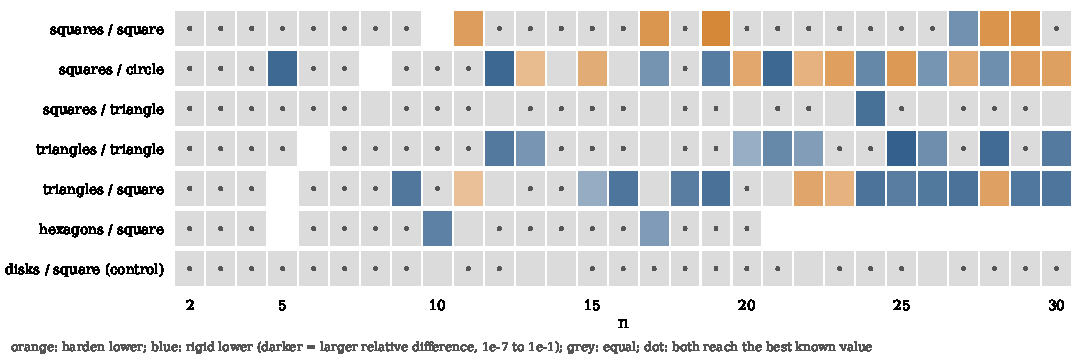
\includegraphics[width=\linewidth]{figures/heatmap}
\caption{Hardening against rigid starts on every instance (C07): which of the two reaches the lower size, and by how much. Blank cells were held out for tuning.}\label{fig:heatmap}
\end{figure}

\paragraph{How often does a method get there?} A count of instances hides how close each call was. Figure~\ref{fig:heatmap} shows every instance: most instances are ties; squares in a square is the only family where every instance but one that differs favours hardening, triangles lean towards rigid starts, and squares in a circle alternate. Figure~\ref{fig:bestofk} shows, for six instances, the share of $k$-run subsets of the observed 32 runs that include a run reaching the best known value. Hardening reaches Trump's $n=11$ and Wainwright's $n=19$ packings in 2 and 3 of 32 runs, and rigid starts in none; on triangle instances the picture is reversed. At $k=32$ the curve is 1 whenever any run succeeded, which says nothing about a fresh batch. Repeated batches do: on the \BatN{} instances of C13, harden and rigid each have three independent 32-run batches at the base budget, and hardening reaches Trump's $n=11$ packing in \BatSqElevenH{} of 3 batches and Schadt's $n=29$ packing in \BatSqTwentyNineH{} of 3, rigid starts in \BatSqElevenR{} and \BatSqTwentyNineR; on the triangles-in-triangle instance $n=29$ it is the other way round (hardening \BatTriTwentyNineH{} of 3, rigid \BatTriTwentyNineR). Over all \BatN{} instances, the best known value is reached in \BatHReached{} of the $3\times\BatN$ hardening batches and \BatRReached{} of the rigid ones, and on \BatHSome{} (harden) and \BatRSome{} (rigid) instances some batches reach it and others do not. Statements that one method is ``the only one'' to reach a packing are statements about one batch of 32 runs.

\begin{figure}[t]\centering
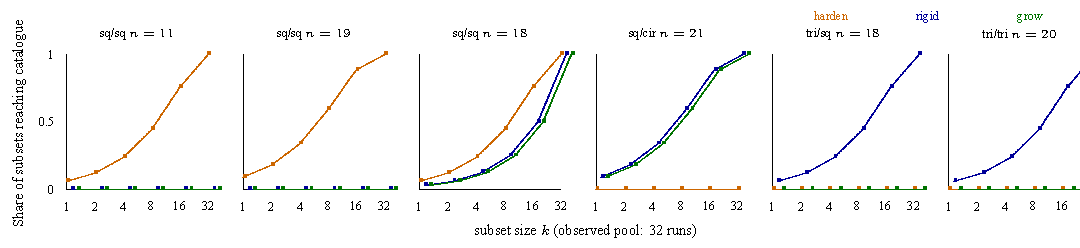
\includegraphics[width=\linewidth]{figures/bestofk}
\caption{Share of $k$-run subsets of the observed 32 runs (C07) that include a run reaching the best known value, $1-\binom{32-s}{k}/\binom{32}{k}$ for $s$ successful runs, on six instances where the gradient paths differ. This is a without-replacement estimate from one pool; it is 1 at $k=32$ whenever $s>0$. Runs not selected for tightening count with their legalised size.}\label{fig:bestofk}
\end{figure}

\paragraph{Inference scope.} The unit of the paired summaries is an instance in a designed benchmark, not an independently sampled application. Families share geometry and the experiments include selected follow-ups. Multiple family/endpoint comparisons and exploratory analyses are therefore interpreted descriptively; nominal sign-test values do not provide family-wide error control. A best-of-32 result is one realization of a restart procedure, and seed-pool resampling cannot establish reliability on new instances or independent batches. Ties and catalogue tolerances are defined by the saved analysis code. No nonsignificant test is treated as evidence of equivalence.

\section{What we learned}\label{sec:learned}
\paragraph{Where hardening differs.} For squares in a square, hardening's lowest size is the lowest of all methods on \CsevenSquInSquHardenLowest{} of \CsevenSquInSquN{} instances and the only one that low on \CsevenSquInSquHardenSole{}; with identical settings, rigid starts manage \CsevenSquInSquRigidLowest{}. In 32 runs each, hardening alone reaches Trump's $n=11$ and Wainwright's $n=19$ packings (Figure~\ref{fig:strip}). For triangles the order reverses: rigid starts are lowest on \CsevenTriInSquRigidLowest{} instances of triangles in a square against \CsevenTriInSquHardenLowest{} for hardening, and \CsevenTriInTriRigidLowest{} against \CsevenTriInTriHardenLowest{} in a triangle (Figure~\ref{fig:tristrip}). On the control family the gradient paths reach the lowest size on the same number of instances, as they should.

\paragraph{With more time on squares.} Campaign C16, a targeted follow-up planned after C07 and C09, tested at ten times the base budget the advantage already seen on squares in a square ($n=17$--$30$, 16 runs per method; Table~\ref{tab:long}). Hardening's lowest size is the lowest of the five on \LongHardenLowest{} of \LongN{} instances (annealing \LongSaLowest, rigid \LongRigidLowest, grow \LongGrowLowest, pc \LongPcLowest), and it reaches the best known value on \LongHardenReached{} (annealing \LongSaReached, rigid \LongRigidReached). Within this 16-run-per-method C16 comparison, hardening is the only method to reach the best known packing for $n=\LongHardenOnlyReachedNs$; annealing is the only one for $n=\LongSaOnlyReachedNs$. Tightening the best run of every method at the four hardening-only instances, regardless of the tightening gate, leaves every other method short of the best known value (\texttt{scripts/c16\_equal\_tighten.py}). Against rigid starts hardening is lower on \LongHLower{} instances and higher on \LongRLower{} ($p=\LongP$), but the hardening and rigid runs at $n=19$, 28 and 29 repeat C09's exactly (same seeds and budget, deterministic runs), and all three are hardening wins; on the remaining \LongNewN{} instances the count is \LongNewHLower{} against \LongNewRLower{} ($p=\LongNewP$). C16 adds new successes against all four other methods at \LongHardenOnlyReachedNewNs{} rather than six independent confirmations.

\IfFileExists{tables/C16.tex}{\begin{table}[t]\centering\small
\begin{tabular}{rrccccc}
\toprule
$n$ & best known & harden & grow & rigid & sa & pc \\
\midrule
17 & 4.67553 & \textbf{\checkmark} & 0.324 & 0.032 & 0.032 & 0.092 \\
18 & 4.82288 & \textbf{\checkmark} & 0.177 & \textbf{\checkmark} & \textbf{\checkmark} & 0.015 \\
19$^\dagger$ & 4.88562 & \textbf{\checkmark} & 0.114 & 0.114 & 0.114 & 0.114 \\
20 & 5.00000 & \textbf{\checkmark} & \textbf{\checkmark} & \textbf{\checkmark} & \textbf{\checkmark} & \textbf{\checkmark} \\
21 & 5.00000 & \textbf{\checkmark} & \textbf{\checkmark} & \textbf{\checkmark} & \textbf{\checkmark} & \textbf{\checkmark} \\
22 & 5.00000 & \textbf{\checkmark} & \textbf{\checkmark} & \textbf{\checkmark} & \textbf{\checkmark} & \textbf{\checkmark} \\
23 & 5.00000 & \textbf{\checkmark} & \textbf{\checkmark} & \textbf{\checkmark} & \textbf{\checkmark} & \textbf{\checkmark} \\
24 & 5.00000 & \textbf{\checkmark} & \textbf{\checkmark} & \textbf{\checkmark} & \textbf{\checkmark} & \textbf{\checkmark} \\
25 & 5.00000 & \textbf{\checkmark} & \textbf{\checkmark} & \textbf{\checkmark} & \textbf{\checkmark} & 0.756 \\
26 & 5.62132 & \textbf{\checkmark} & 0.379 & 0.379 & 0.086 & 0.202 \\
27 & 5.70711 & 0.098 & 0.293 & 0.139 & \textbf{\checkmark} & 0.294 \\
28$^\dagger$ & 5.82444 & \textbf{0.042} & 0.176 & 0.073 & 0.178 & 0.179 \\
29$^\dagger$ & 5.93383 & \textbf{\checkmark} & 0.066 & 0.066 & 0.066 & 0.066 \\
30 & 6.00000 & \textbf{\checkmark} & \textbf{\checkmark} & \textbf{\checkmark} & \textbf{\checkmark} & \textbf{\checkmark} \\
\bottomrule
\end{tabular}
\caption{Squares in a square at ten times the base budget (C16, 16 runs per method). Y: reaches the catalogue value within tolerance; otherwise the gap to it. Bold: lowest of the five. $^\dagger$: hardening and rigid runs repeat C09 exactly (same seeds and budget, deterministic runs).}
\label{tab:long}
\end{table}
}{}

\paragraph{Separating the disk start from the gradual path.} Hardening differs from rigid starts in two ways: pieces are compressed as disks, and they then harden gradually. Campaign C11 separates the two with \emph{snap}, which compresses disks exactly as hardening does and then switches to the polygons in one step, with the same seeds, settings and budget (Table~\ref{tab:ablate}). Its pre-registered test compares, per family, the instances that exactly one of harden and snap solves. On squares in a square only two instances are discordant, so the test is inconclusive ($p=0.5$). The plan's decision rule then attributed hardening's advantage there to the disk-compressed start. That rule was wrong: failing to detect a difference does not show that there is none, still less which mechanism is responsible. We record the rule and its output, and draw no causal conclusion from it.

Exploratory comparisons of the sizes reached, which were not the pre-registered test, are as follows. We detect no difference between snap and rigid starts (each lower on \SnapRXLower{} and \SnapRRLower{} of \CsevenInstances{} instances). Hardening and snap differ in opposite directions by family: counting instances where hardening is lower against those where snap is lower, squares in a square give \SnapSquSqu{}, triangles in a triangle \SnapTriTri{} and triangles in a square \SnapTriSqu{} (all families, \SnapHLower{} against \SnapXLower, $p=\SnapP$). The pooled exploratory lowest-size comparison favors snap (17 hardening-lower versus 36 snap-lower, $p=0.0126603$), opposite to the square-in-square direction (6 versus 0). These are family-dependent descriptive differences; they do not identify a causal orientation mechanism. A confirmatory directional test on squares would need more discordant instances than the registered reached-endpoint comparison provides.

Campaign C12 asks the same of area. A hardening piece also grows, by up to 40\% of its area; \emph{grow-area} keeps rigid polygons but scales them so their area follows hardening's schedule exactly. Again we detect no difference from rigid starts (lower on \AreaRXLower{} and \AreaRRLower{} instances), and hardening differs from it in the same directions as from snap: \AreaSquSqu{} on squares in a square and \AreaTriTri{} on triangles in a triangle (all families \AreaHLower{} against \AreaXLower, $p=\AreaP$). Its registered reached-endpoint test on squares in a square has 2 hardening-only versus 0 grow-area-only successes ($p=0.5$), again inconclusive; the 5 versus 1 lowest-size comparison ($p=0.21875$) is exploratory. Neither the disk start nor the area schedule alone reproduces hardening's pattern of results.

\begin{table}[t]\centering\small
\begin{tabular}{lrcccc}
\toprule
family & $N$ & harden : snap & snap : rigid & harden : grow-area & grow-area : rigid \\
\midrule
squares in square & 28 & 6 : 0 & 1 : 2 & 5 : 1 & 2 : 1 \\
squares in circle & 28 & 5 : 11 & 10 : 6 & 9 : 8 & 8 : 4 \\
squares in triangle & 29 & 0 : 1 & 0 : 0 & 0 : 1 & 0 : 0 \\
triangles in triangle & 28 & 0 : 8 & 0 : 2 & 1 : 8 & 0 : 3 \\
triangles in square & 28 & 6 : 14 & 8 : 9 & 5 : 11 & 5 : 6 \\
hexagons in square & 18 & 0 : 2 & 1 : 1 & 0 : 2 & 0 : 0 \\
disks in square & 29 & 0 : 0 & 0 : 0 & 0 : 0 & 0 : 0 \\
\midrule all & 188 & 17 : 36 & 20 : 20 & 20 : 31 & 15 : 14 \\
\bottomrule
\end{tabular}
\caption{Which part of hardening matters (C11, C12; harden and rigid from C07, same seeds, settings and budget). Each cell $a:b$ counts the instances on which the first method\textquotesingle s lowest size is lower than the second\textquotesingle s, and the reverse; the rest are ties. \emph{snap} compresses disks as hardening does, then switches to polygons at once; \emph{grow-area} keeps rigid polygons whose area follows hardening\textquotesingle s.}
\label{tab:ablate}
\end{table}


\paragraph{What the pieces do.} Figure~\ref{fig:mechanism} measures three things on the replay of each instance's best run (lowest legalised size, before tightening), for hardening and rigid starts: net displacement of pieces between the end of compression and the end of the run, net rotation over the same interval, and the share of pieces that end tilted against every container edge. Midway through the morph phase, where a hardening piece has $\tau\approx0.5$, the orientational order of squares in a square, $|\langle e^{4i\theta}\rangle|$, has a median of \MechSquSquHardenOrder{}; at the same step of a rigid run it is \MechSquSquRigidOrder, so rigid squares are more aligned at that point than hardening squares. On the \MechSoleN{} squares-in-square instances where hardening alone reaches the lowest size, its final packing has more tilted squares than rigid's best on the same instance every time (\MechSoleMore{} of \MechSoleN; median shares \MechSoleTiltH{} against \MechSoleTiltR), as the classical packings at $n=11$, 17 and 19 require. On triangles in a triangle hardening pieces move about twice as far after compression as rigid ones (median \MechTriTriHardenMove{} against \MechTriTriRigidMove{} unit sides), and on the \MechTriFailN{} instances where rigid starts alone reach the lowest size the gap is the same (\MechTriFailMoveH{} against \MechTriFailMoveR). These are descriptive. They fit two hypotheses: that the support function's factor $1-\tau$ lets hardening defer the choice of orientation until neighbours are in place, which squares need when a block must tilt against aligned neighbours; and that triangles, whose corners stick out twice as far as their inradius ($R/\rho=2$, against $\sqrt2$ for a square) and whose good packings alternate up and down, pay for that deferral with large rearrangements. The area explanation alone (a triangle's inscribed disk covers 60\% of it, a square's 79\%) is weakened by hexagons, whose disk covers 91\% and where hardening is no better than rigid starts (\CsevenHexInSquHardenLowest{} against \CsevenHexInSquRigidLowest{} of \CsevenHexInSquN{}, mostly ties). Changing the path also changes contact geometry and forces, so none of this isolates orientation as the cause.

\begin{figure}[t]\centering
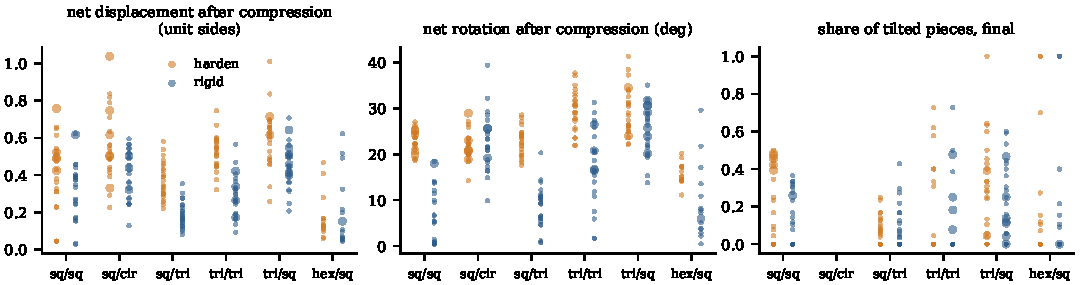
\includegraphics[width=\linewidth]{figures/mechanism}
\caption{What pieces do after compression, on the best run of each C07 instance with $n\ge6$ (orange: hardening; blue: rigid; large dots: the method alone reached the lowest size). Left: mean net displacement; middle: mean net rotation, modulo the piece's symmetry (for hardening this includes turning while pieces are still nearly round and orientation costs almost nothing); right: share of pieces with no edge within $2^\circ$ of a container edge (square and triangle containers).}\label{fig:mechanism}
\end{figure}

\paragraph{Does choosing the path transfer to new families?} If the better path depends on the family, a search could choose it per instance. Campaign C15 tests that as a decision on four families not used for tuning or method analysis: pentagons and octagons in a square, hexagons in a triangle and triangles in a circle, $n=6$--$20$ (\DecN{} instances). Before the plan was written, one geometry smoke-test run at $n=8$, seed 3, was made for each family and path; this exception qualifies the held-out description. Each instance then gets 64 hardening and 64 rigid runs, from which three pre-registered policies of 64 runs are formed: always rigid, always harden, and a pilot that spends 8 runs on each path and the remaining 48 on the path whose pilot reached the lower legalised (untightened) size (Table~\ref{tab:decision}). The pilot and always-rigid rarely differ (lower on \DecPilotLower{} and \DecRigidLower{} instances, $p=\DecP$), so by the plan's rule we report no detected benefit from choosing the path. Always-harden is worse than always-rigid (\DecHLower{} against \DecHRLower, $p=\DecHP$), most clearly on pentagons, and reaches the best known value on \DecReachedHarden{} instances against \DecReachedRigid{} for rigid starts and \DecReachedPilot{} for the pilot. The pilot picked hardening on \DecPicked{} instances and so avoided most of its losses, but was lower than always-rigid on only \DecPilotLower{} instances. The pilot compares untightened sizes, which Table~\ref{tab:refine} shows can misrank methods; in a post-hoc check that compares the tightened best pilot run of each path instead, the pilot picks hardening on \DecTPicked{} instances rather than \DecPicked, changes \DecTChanged{} decisions, and still differs from always-rigid on \DecTLower{} against \DecTRLower{} instances (\texttt{scripts/c15\_tightened\_pilot.py}). None of these families shows a family-level advantage for hardening (it is lower on \DecHLower{} individual instances), so the test says that this pilot policy found no gain on these families; it is not a test of whether a selector can find a favourable family, since none was present.

\IfFileExists{tables/C15.tex}{\begin{table}[t]\centering\small
\begin{tabular}{lrcccc}
\toprule
family & $N$ & harden : rigid & pilot : rigid & pilot chose harden & reached (r / h / p) \\
\midrule
pentagons in square & 15 & 1 : 8 & 0 : 1 & 3 & 8 / 4 / 8 \\
octagons in square & 15 & 0 : 3 & 0 : 0 & 6 & 11 / 9 / 11 \\
hexagons in triangle & 15 & 0 : 2 & 0 : 1 & 8 & 10 / 9 / 10 \\
triangles in circle & 15 & 2 : 4 & 2 : 1 & 3 & 11 / 10 / 12 \\
\midrule
all & 60 & 3 : 17 & 2 : 3 & 20 & 40 / 32 / 41 \\
\bottomrule
\end{tabular}
\caption{Held-out families (C15), $n=6$--$20$, 64 runs per policy. $a:b$ counts instances where the first policy\textquotesingle s result is lower than the second\textquotesingle s and the reverse. The pilot spends 8 runs on each path, then 48 on the one whose pilot went lower. Reached (r / h / p): instances where always-rigid, always-harden and the pilot reach the best known value.}
\label{tab:decision}
\end{table}
}{}

\paragraph{Partly soft starts.} Varying only the starting softness $\tau_0$ on the \CtauN{} most contested instances (Table~\ref{tab:tau}), the counts of instances where each value reaches the lowest size are \CtauOne, \CtauHalf, \CtauQuarter{} and \CtauZero{} for $\tau_0=1, 0.5, 0.25, 0$. Squares in a square favour soft starts (\CtauSquares{}); triangles favour rigid or slightly rounded ones (\CtauTriangles{}). These instances were selected where hardening and rigid starts disagreed, mostly in rigid's favour, which tilts this count toward small $\tau_0$; partly rounded starts are a candidate default, not an established one.

\begin{table}[t]\centering\small
\begin{tabular}{lrrrrr}
\toprule
family & instances & $\tau_0=1$ (harden) & $0.5$ & $0.25$ & $0$ (rigid)\\
\midrule
squares in square & 6 & 3 & 4 & 2 & 0\\
squares in circle & 13 & 2 & 3 & 6 & 5\\
squares in triangle & 1 & 0 & 1 & 1 & 1\\
triangles in triangle & 7 & 0 & 4 & 3 & 5\\
triangles in square & 12 & 2 & 3 & 5 & 5\\
hexagons in square & 1 & 0 & 0 & 1 & 1\\
\midrule
all & 40 & 7 & 15 & 18 & 17\\
\bottomrule
\end{tabular}
\caption{How soft the start must be (C08): on the 40 most contested instances of C07, the number of instances where each starting softness $\tau_0$ reaches the lowest size (32 runs each, all other settings equal; ties counted for every tied value).}
\label{tab:tau}
\end{table}


\paragraph{Longer runs, or more runs?} An earlier test (C09, appendix) suggested that hardening gains more than rigid starts from longer schedules, but it changed run length and restart count together and used instances chosen because the two paths disagreed. Campaign C13 repeats it cleanly on \BudN{} instances fixed in advance ($n=11,17,23,29$ per family; hexagons $n=8,12,16,20$), with 32 runs at three times the budget, and 96 runs at the base budget for the same nominal total step allocation. Counting instances where hardening is lower against those where rigid starts are lower: \BudOneH{} against \BudOneR{} with 32 base runs ($p=\BudOneP$), \BudThreeH{} against \BudThreeR{} with 32 long runs, and \BudMoreH{} against \BudMoreR{} with 96 base runs. Longer runs improved rigid starts more than hardening (rigid lower than its base on \BudGainR{} instances and higher on \BudLossR; hardening \BudGainH{} and \BudLossH), and at equal nominal step allocation, three times longer runs and three times as many runs did about equally well for both paths (\BudLvMLH{} against \BudLvMMH{} for hardening, \BudLvMLR{} against \BudLvMMR{} for rigid). The C09 result does not replicate; we withdraw it.

\paragraph{Two paths, or more runs of one?} The paths fail on different families, so running both might help. At equal total budget, 32 rigid runs plus 32 hardening runs solve \PortRigidHarden{} of the \CsevenInstances{} instances, against \PortRigidSixtyFour{} for 64 rigid runs and \PortRigidGrow{} for 32 rigid plus 32 growing runs (instances solved by exactly one of the first two: \PortSign, two-sided $p=\PortP$). On squares in a square alone the mixed portfolio solves one instance more than doubled rigid runs: it gains $n=11$ and 19 and loses $n=27$. The C10 plan specified a one-sided sign test; its report gives $p=\CtenRegisteredP$, whereas the two-sided descriptive value reported here is $p=\PortP$. We detected no benefit from this allocation. These data establish neither an advantage nor equivalence. Equal total budget here means nominal run/step allocation, not equal complete CPU time including tuning and tightening.

\paragraph{Tuning decides comparisons.} Our first experiments compared hardening with rigid starts that inherited the hardening schedule, on two square instances, and hardening looked better. Tuned with comparable effort, rigid starts led overall. Re-tuning for the lowest point instead of the median changed four of the five methods' settings (stronger pressure for the gradient paths, more noise for rigid starts) and helped simulated annealing most. It kept the broad pattern, hardening for squares in a square and rigid or growing starts for triangles, though the leading method changed for squares in a circle and triangles in a square.

\section{When to use it, and downstream use}\label{sec:matters}
\paragraph{When to add hardening.} Under these in-house implementations, tested settings and budgets, rigid starts remain the better default. Hardening is a candidate additional path on squares in a square, where it reached packings none of the other four methods reached (Section~\ref{sec:learned}) and where the methods cover different instances: at ten times the budget, hardening and annealing together reach every best known value from $n=17$ to 30 except $n=28$. Our hypothesis is that it helps where good packings tilt a block of pieces against an otherwise aligned arrangement, but that is not a validated predictor: we have no test that identifies favourable families in advance, and we have not shown that splitting a fixed budget between hardening and rigid starts beats spending it on rigid starts (C10). The tested settings favor rigid starts on triangles and the additional families; this evidence does not support replacing them with hardening as a default.

\paragraph{Downstream use.} The earlier cube release \citep{softtorigidpacking} has been reused by others; we report this separately from our results, which it does not change. A continuation of the unfinished $n=13$ cube search \citep{n13repo} builds on our simulator, reuses our tightening code and checkers unchanged, adds two moves (re-melting a finished packing: soften, expand slightly, reharden; and inserting a thirteenth cube into the 12-cube packing), and after 2{,}627 runs reports a certified packing of side $2.956149$ at $10^{-6}$ clearance, consistent with Friedman's $2.956+$ and not claimed as an improvement; C05 reaches a comparable numerical contact value ($2.956145$) without clearance. \citet{platonicrepo} generalises the construction to all five Platonic solids as pieces and containers, with exact feasibility checks over $\mathbb{Q}(\sqrt2,\sqrt5)$ and an archive search that repeatedly softens and rehardens existing packings; the reported values are certified upper bounds, and comparisons with \citet{Berthold2026} must convert between edge and circumradius normalisations. \citet{tesseractrepo} reimplements ball-to-hypercube continuation independently in four dimensions and combines it with structured seeds, constrained polishing and basin hopping, reporting floating-point candidates for 26--30 tesseracts. Together they continue a partially explored search, extend the geometry and the exact verification to new solids, and reimplement the method in a higher dimension. None is a controlled comparison, and the first two inherit our simulator (one modified, one generalised) and tightening scheme, so they are not independent validations of it; the generalised exact checker is new verification work. What they add is a use we did not test: softening as a rearrangement operator inside a larger search rather than only as a cold start. Whether temporary softening escapes a rigid local optimum better than rigid perturbation at equal budget, from shared starting packings, is the experiment they motivate.

\paragraph{Other settings.} The same question arises wherever an overlap penalty is minimised in a shrinking container: irregular nesting \citep{Wascher2007,Bennell2008,Leao2020}, where inscribed circles are already an overlap proxy \citep{Jones2014,Gardeyn2025}; floorplanning, where circles-then-rectangles is an established two-stage switch \citep{AnjosVannelli2002,Luo2008}; and faceted particles in confinement \citep{Torquato2018,Wang2018}. In each, C11 is the test to run first, and real objectives add stability, orientation and ordering constraints \citep{Bortfeldt2013,Araujo2019} that any gain in density must survive.

\section{Limitations and open directions}\label{sec:limits}
\paragraph{Limitations.} These are search results, not optimality proofs, and tightening is a local method. In the main comparison (C07) each instance had 32 runs per method at a fixed budget, and C16 had 16; ``only one method reached it'' holds within the run count and budget stated for that campaign. Gradient paths are matched in steps, not pair evaluations or wall-clock time (hardening was the fastest per run in the two square-in-square diagnostic cells); the baselines are matched to a hardening run's pair evaluations, which perturbation--compression overshoots (Table~\ref{tab:diag}). Simulated annealing and perturbation--compression are our implementations; their best runs were less often close enough to be tightened, so the tightening policy favours the gradient paths, most for pc (C14 shows the order survives equal tightening on 28 instances); in C16 the other methods' best runs at the hardening-only instances were tightened after the fact and remained short of the best known value. The lowest-point tuning used instances larger than the test set, and in that round all five winners sat at corners of their two-axis grids and the grid was not extended. Comparable grid effort is not proof of comparable tuning adequacy; simulated annealing moved furthest between the two tuning rounds, so its results are best read as a lower bound on what a wider grid would give. Its step size adapts every 200 moves to keep the acceptance rate between 20\% and 40\%, so at $T_0=10^{-3}$ it behaves as a Metropolis walk with small adaptive steps rather than one with large uphill moves. The grids' ranges were first chosen during development on squares in a square, and settings suited to triangles could lie outside them; the C08 sweep of starting softness is only a partial check. In 3D only the three gradient paths were compared. Catalogue values come from captions and witnesses as of October 2026; truncated values are only known to their printed precision. Not detecting a difference (between mixed and single-path portfolios, between snap or grow-area and rigid starts, or between the pilot and always-rigid) is not evidence of equivalence at these sample sizes.

\paragraph{Open directions.}
\begin{itemize}\itemsep1pt
\item \emph{A rule that predicts the path.} The pilot showed no detected benefit on held-out families that had no aggregate hardening advantage. A useful rule would have to predict, before running, the families where it does; we have one such family and no rule that singles it out in advance.
\item \emph{External baselines.} Our simulated annealing and perturbation--compression are our own implementations. Published alternatives require a compatibility audit before a fair comparison. \citet{Berthold2026} provide regular-polygon/container and cube variants that can be compared after explicit scale conversion; their Section~4 variable-radius, maximum-sum circle objective does not match our congruent-disk control; their Section~5 unit-circle/variable-ellipse model is a different container problem. Sparrow \citep{Gardeyn2025} minimizes strip length at fixed width rather than the finite container scale studied here; adapting that objective would be a changed experiment. No external competitiveness claim is made without such a matched test.
\item \emph{Softening as a move.} Re-softening an existing packing and rehardening it, as downstream searches do \citep{n13repo,platonicrepo}, against rigid perturbation from the same packings at equal budget.
\item \emph{Other paths.} Paths through other shape families (an ellipse for a rectangle, a rounded octahedron for a cube, superellipses \citep{Jiao2008}), paths that harden pieces one at a time, or schedules that adapt $\tau$ to the current overlap.
\item \emph{Larger $n$, other solids, other solvers.} Most unsolved instances have $n\ge17$. Our controlled study did not include solids other than cubes; downstream work now explores them \citep{platonicrepo} and higher dimensions \citep{tesseractrepo}, without controlled baselines. Hardening could also seed exact models \citep{Berthold2026} or shrink-and-separate nesters \citep{Gardeyn2025}.
\item \emph{Non-convex and mixed pieces.} The rounded-shape construction needs a convex core; non-convex pieces would need a different family of intermediate shapes, for example a convex decomposition hardened part by part.
\end{itemize}



\sloppy
\section*{Statements and Declarations}
\paragraph{Data and code availability.} Study code, campaign plans, raw run outputs, saved analyses and selected replays are available at \url{https://github.com/yoheinakajima/soft-to-rigid/tree/07e3cbd3c4855e5e19344885fbf672c3d7a0f039}. The original event export covers C00--C10; later analyses also read versioned campaign files directly. Online Resource 1 describes the evidence map, limitations of certification and a saved-output verification route. A new optimizer campaign is not needed to inspect the reported stored results. Code is distributed under the repository's MIT license; third-party records and witnesses retain their respective rights. A versioned preparation manifest accompanies this draft.
\paragraph{Funding and competing interests.} Author confirmation pending. No absence of funding, financial interests or nonfinancial interests is asserted by this draft.
\paragraph{Author contributions and approval.} The public v1 names Yohei Nakajima as sole author. Contributions, author details and approval of this journal draft must be confirmed before submission.
\paragraph{Ethics and consent.} The reported experiments concern computational geometry rather than human or animal participants. The corresponding not-applicable declarations remain subject to author confirmation.
\paragraph{AI assistance.} The public study acknowledges that code, experiments and verification were developed with Claude (Anthropic) under the author's direction. This journal preparation draft was edited and audited with Codex (OpenAI). Exact tool/version/date details and the human verification performed must be confirmed by the author before submission. AI systems are not authors; responsibility and approval remain with the human author. This assistance is substantive and is not represented as copy editing alone.
\paragraph{Related work and overlap.} Public v1 is \url{https://arxiv.org/abs/2610.14463v1}, distributed under CC BY 4.0. The earlier twelve-cube note is described in the public bibliography as submitted to Geombinatorics; current editorial status, permissions and overlap clearance are unverified. The draft distinguishes that prior discovery from the present controlled study. No assertion of exclusive consideration is made until the author confirms current status.

\FloatBarrier
\bibliographystyle{plainnat}
\setlength{\bibsep}{1pt plus 0.3ex}
\renewcommand{\bibfont}{\footnotesize}
\bibliography{refs}

\clearpage
\appendix
\section{Campaign and diagnostic details}
\suppressfloats[t]

\paragraph{Campaigns.} C00 reproduce the earlier square results; C01--C03 median tuning; C04 breadth (median-tuned); C05 cubes; C06 lowest-point tuning; C07 breadth (lowest-point-tuned, main); C08 starting softness; C09 longer schedules (confounded); C10 portfolio; C11 snap; C12 grow-area; C13 clean budget study; C14 equal tightening; C15 held-out families (path choice); C16 squares in a square at ten times the budget. Plans, amendments, raw runs, reports and the decision recorded for each are in \texttt{campaigns/} and the journal.

\paragraph{Frozen settings.} Median-tuned (C01--C03): harden $\mu=0.08$, noise $\times8$; grow $\mu=0.04$, $\gamma_0=0.2$; rigid $\mu=0.04$, noise $\times2$; sa $T_0=3\cdot10^{-3}$, $\mu=0.0025$; pc kick $0.05$, relax $19200$ steps. Lowest-point-tuned (C06): harden and rigid $\mu=0.16$, noise $\times8$; grow $\mu=0.08$, $\gamma_0=0.1$; sa $T_0=10^{-3}$, $\mu=0.02$; pc kick $0.05$, relax $19200$ steps. All are in \texttt{methods/*.json}, each with the campaign and grid point that selected it.

\paragraph{Longer schedules, first attempt (C09).} C09 gave hardening and rigid starts three and ten times the budget on the \CbudgetN{} instances where the two differed most. It changed run length and restart count together (32 runs at budget 1, 16 at budgets 3 and 10) and selected instances for disagreement, mostly in rigid's favour, so part of its change is regression toward an even split. We report it (Table~\ref{tab:budget}) but draw conclusions about run length only from C13, which fixes these confounds.
\begin{table}[t]\centering\small
\begin{tabular}{rrrrr}
\toprule
budget & harden lowest & rigid lowest & harden reaches best known & rigid reaches best known\\
\midrule
1$\times$ & 3 & 17 & 1 & 10\\
3$\times$ & 5 & 16 & 2 & 10\\
10$\times$ & 9 & 16 & 6 & 9\\
\bottomrule
\end{tabular}
\caption{Longer schedules (C09) on the 20 most contested instances: number of instances where each path reaches the lower of the two lowest sizes (ties counted for both), and where it reaches the best known value. Budget 1 is C07 (32 runs); budgets 3 and 10 use 16 runs.}
\label{tab:budget}
\end{table}


Figure~\ref{fig:gaps} shows per-instance lowest sizes relative to the catalogue.
\begin{table}[t]\centering\small
\begin{tabular}{lrccccc}
\toprule
family & $N$ & \textbf{harden} & \textbf{grow} & \textbf{rigid} & \textbf{sa} & \textbf{pc} \\
\midrule
squares in square & 28 & \textbf{28 (7)} & 21 & 20 & 10 & 17 \\
squares in circle & 28 & 16 (7) & 11 (2) & \textbf{19 (9)} & 10 & 8 \\
squares in triangle & 29 & 27 & 24 & \textbf{29 (1)} & 13 & 7 \\
triangles in triangle & 28 & 19 (1) & 22 (3) & \textbf{24 (4)} & 8 & 10 \\
triangles in square & 28 & 10 (1) & \textbf{19 (5)} & 18 (7) & 12 (1) & 5 \\
hexagons in square & 18 & 15 & 15 (1) & \textbf{17 (2)} & 8 & 6 \\
circles in square (control) & 29 & 27 & 27 & \textbf{28} & 11 (1) & 11 \\
\midrule
all & 188 & 142 (16) & 139 (11) & \textbf{155 (23)} & 72 (2) & 64 (0) \\
reached best known & & 121 & 119 & 132 & 69 & 63 \\
\bottomrule
\end{tabular}
\caption{Settings tuned by median gap (C04). Same layout as Table~\ref{tab:main}.}
\label{tab:median}
\end{table}

\begin{table}[ht]\centering\small
\begin{tabular}{lrrrrrrr}
\toprule
method & \multicolumn{2}{c}{steps (sa: moves) per run} & \multicolumn{2}{c}{pair evaluations per run} & \multicolumn{2}{c}{ms per run} & best run \\
 & $n=20$ & $n=30$ & $n=20$ & $n=30$ & $n=20$ & $n=30$ & tightened \\
\midrule
harden & 11{,}500 & 11{,}500 & 418{,}365 & 650{,}532 & 451 & 699 & 97\% \\
grow & 11{,}500 & 11{,}500 & 426{,}807 & 668{,}192 & 727 & 1{,}183 & 98\% \\
rigid & 11{,}500 & 11{,}500 & 348{,}285 & 550{,}494 & 633 & 1{,}001 & 100\% \\
sa & 66{,}854 & 104{,}043 & 448{,}878 & 714{,}120 & 582 & 983 & 94\% \\
pc & 19{,}148 & 20{,}530 & 690{,}285 & 1{,}176{,}434 & 1{,}117 & 1{,}993 & 56\% \\
\bottomrule
\end{tabular}
\caption{Work per run (C07, squares in a square, mean over 32 runs), wall-clock milliseconds per run on one core (Node.js), and the share of instances on which each method's best run was within 2\% of the best known value and so was tightened (all families). Gradient paths are matched in steps; the baselines stop once they exceed a reference hardening run's pair evaluations.}\label{tab:diag}
\end{table}


\begin{figure}[t]\centering
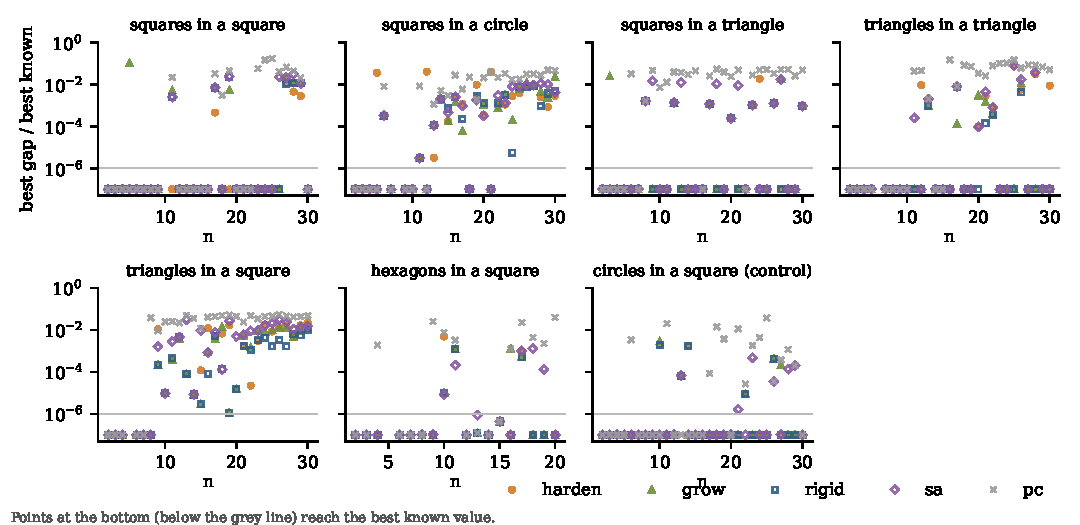
\includegraphics[width=\linewidth]{figures/gaps}
\caption{Lowest size reached per instance and method, relative to the best known value (C07). Points on the bottom row reach it.}\label{fig:gaps}
\end{figure}

\end{document}
